% Soubory musí být v kódování, které je nastaveno v příkazu \usepackage[...]{inputenc}

\documentclass[%        Základní nastavení
%  draft,    				  % Testovací překlad
  12pt,       				% Velikost základního písma je 12 bodů
  a4paper,    				% Formát papíru je A4
  oneside,      			% Jednostranný tisk
	%twoside,      			% Dvoustranný tisk (kapitoly a další důležité části tedy začínají na lichých stranách)
	unicode,						% Záložky a metainformace ve výsledném  PDF budou v kódování unicode
]{report}				    	% Dokument třídy 'zpráva', vhodná pro sazbu závěrečných prací s kapitolami

\usepackage[utf8]		  %	Kódování zdrojových souborů je UTF-8
	{inputenc}					% Balíček pro nastavení kódování zdrojových souborů

\usepackage[				% Nastavení geometrie stránky
	bindingoffset=10mm,		% Hřbet pro vazbu
	hmargin={25mm,25mm},	% Vnitřní a vnější okraj
	vmargin={25mm,34mm},	% Horní a dolní okraj
	footskip=17mm,			  % Velikost zápatí
	nohead,					      % Bez záhlaví
	marginparsep=2mm,		  % Vzdálenost marginálií
	marginparwidth=18mm,	% Šířka marginálií
]{geometry}

\usepackage{sectsty}
	%přetypuje nadpisy všech úrovní na bezpatkové, kromě \chapter, která je přenastavena zvlášť v thesis.sty
	\allsectionsfont{\sffamily}

\usepackage{graphicx} % Balíček 'graphicx' pro vkládání obrázků
											% Nutné pro vložení logotypů školy a fakulty

\usepackage[          % Balíček 'acronym' pro sazby zkratek a symbolů
	nohyperlinks				% Nebudou tvořeny hypertextové odkazy do seznamu zkratek
]{acronym}						
											% Nutné pro použití prostředí 'acronym' balíčku 'thesis'

\usepackage[
	breaklinks=true,		% Hypertextové odkazy mohou obsahovat zalomení řádku
	hypertexnames=false % Názvy hypertext. odkazů budou tvořeny nezávisle na názvech TeXu
]{hyperref}						% Balíček 'hyperref' pro sazbu hypertextových odkazů
											% Nutné pro použití příkazu 'pdfsettings' balíčku 'thesis'

\usepackage{pdfpages} % Balíček umožňující vkládat stránky z PDF souborů
                      % Nutné při vkládání titulních listů a zadání přímo
                      % ve formátu PDF z informačního systému

\usepackage{enumitem} % Balíček pro nastavení mezerování v odrážkách
  \setlist{topsep=0pt,partopsep=0pt,noitemsep} % konkrétní nastavení

\usepackage{cmap} 		% Balíček cmap zajišťuje, že PDF vytvořené `pdflatexem' je
											% plně "prohledávatelné" a "kopírovatelné"

%\usepackage{upgreek}	% Balíček pro sazbu stojatých řeckých písmem
											%% např. stojaté pí: \uppi
											%% např. stojaté mí: \upmu (použitelné třeba v mikrometrech)
											%% pozor, grafická nekompatibilita s fonty typu Computer Modern!
                      
%\usepackage{amsmath} %balíček pro sabu náročnější matematiky                 

\usepackage{dirtree}	% sazba adresářové struktury
                      % vhodné pro prezentaci obsahu elektronické přílohy (např. CD)

\usepackage[formats]{listings}	% Balíček pro sazbu zdrojových textů
\lstset{              % nastavení
%	Definice jazyka použitého ve výpisech
%    language=[LaTeX]{TeX},	% LaTeX
%	language={Matlab},		% Matlab
	language={C},           % jazyk C
    basicstyle=\ttfamily,	% definice základního stylu písma
    tabsize=2,			% definice velikosti tabulátoru
    inputencoding=utf8,         % pro soubory uložené v kódování UTF-8
		columns=fixed,  %fixed nebo flexible,
		fontadjust=true %licovani sloupcu
    extendedchars=true,
    literate=%  definice symbolů s diakritikou
    {á}{{\'a}}1
    {č}{{\v{c}}}1
    {ď}{{\v{d}}}1
    {é}{{\'e}}1
    {ě}{{\v{e}}}1
    {í}{{\'i}}1
    {ň}{{\v{n}}}1
    {ó}{{\'o}}1
    {ř}{{\v{r}}}1
    {š}{{\v{s}}}1
    {ť}{{\v{t}}}1
    {ú}{{\'u}}1
    {ů}{{\r{u}}}1
    {ý}{{\'y}}1
    {ž}{{\v{z}}}1
    {Á}{{\'A}}1
    {Č}{{\v{C}}}1
    {Ď}{{\v{D}}}1
    {É}{{\'E}}1
    {Ě}{{\v{E}}}1
    {Í}{{\'I}}1
    {Ň}{{\v{N}}}1
    {Ó}{{\'O}}1
    {Ř}{{\v{R}}}1
    {Š}{{\v{S}}}1
    {Ť}{{\v{T}}}1
    {Ú}{{\'U}}1
    {Ů}{{\r{U}}}1
    {Ý}{{\'Y}}1
    {Ž}{{\v{Z}}}1
}
\usepackage{listings}
%%%%%%%%%%%%%%%%%%%%%%%%%%%%%%%%%%%%%%%%%%%%%%%%%%%%%%%%%%%%%%%%%
%%%%%%      Definice informací o dokumentu             %%%%%%%%%%
%%%%%%%%%%%%%%%%%%%%%%%%%%%%%%%%%%%%%%%%%%%%%%%%%%%%%%%%%%%%%%%%%

% V tomto souboru se nastavují téměř veškeré informace, proměnné mezi studenty:
% jméno, název práce, pohlaví atd.
% Tento soubor je SDÍLENÝ mezi textem práce a prezentací k obhajobě -- netřeba něco nastavovat na dvou místech.

\usepackage[
%%% Z následujících voleb jazyka lze použít pouze jednu
  %czech-english,		% originální jazyk je čeština, překlad je anglicky (výchozí)
  %english-czech,	% originální jazyk je angličtina, překlad je česky
  slovak-english,	% originální jazyk je slovenština, překlad je anglicky
  %english-slovak,	% originální jazyk je angličtina, překlad je slovensky
%
%%% Z následujících voleb typu práce lze použít pouze jednu
  semestral,		  % semestrální práce (nesází se abstrakty, prohlášení, poděkování) (výchozí)
  %bachelor,			%	bakalářská práce
  %master,			  % diplomová práce
  %treatise,			% pojednání o disertační práci
  %doctoral,			% disertační práce
%
%%% Z následujících voleb zarovnání objektů lze použít pouze jednu
%  left,				  % rovnice a popisky plovoucích objektů budou zarovnány vlevo
	center,			    % rovnice a popisky plovoucích objektů budou zarovnány na střed (vychozi)
%
]{thesis}   % Balíček pro sazbu studentských prací


%%% Jméno a příjmení autora ve tvaru
%  [tituly před jménem]{Křestní}{Příjmení}[tituly za jménem]
% Pokud osoba nemá titul před/za jménem, smažte celý řetězec '[...]'
\author{Samuel Kopecký}{}

%%% Identifikační číslo autora (VUT ID)
\butid{007}

%%% Pohlaví autora/autorky
% (nepoužije se ve variantě english-czech ani english-slovak)
% Číselná hodnota: 1...žena, 0...muž
\gender{0}

%%% Jméno a příjmení vedoucího/školitele včetně titulů
%  [tituly před jménem]{Křestní}{Příjmení}[tituly za jménem]
% Pokud osoba nemá titul před/za jménem, smažte celý řetězec '[...]'
\advisor[doc.\ Ing.]{Křestní}{Příjmení}[Ph.D.]


%%% Jméno a příjmení oponenta včetně titulů
%  [tituly před jménem]{Křestní}{Příjmení}[tituly za jménem]
% Pokud osoba nemá titul před/za jménem, smažte celý řetězec '[...]'
% Nastavení oponenta se uplatní pouze v prezentaci k obhajobě;
% v případě, že nechcete, aby se na titulním snímku prezentace zobrazoval oponent, pouze příkaz zakomentujte;
% u obhajoby semestrální práce se oponent nezobrazuje (jelikož neexistuje)
% U dizertační práce jsou typicky dva až tři oponenti. Pokud je chcete mít na titulním slajdu, prosím ručně odkomentujte a upravte jejich jména v definici "VUT title page" v souboru thesis.sty.
%\opponent[doc.\ Mgr.]{Křestní}{Příjmení}[Ph.D.]

%%% Název práce
%  Parametr ve složených závorkách {} je název v originálním jazyce,
%  parametr v hranatých závorkách [] je překlad (podle toho jaký je originální jazyk).
%  V případě, že název Vaší práce je dlouhý a nevleze se celý do zápatí prezentace, použijte příkaz
%  \def\insertshorttitle{Zkác.\ náz.\ práce}
%  kde jako parametr vyplníte zkrácený název. Pokud nechcete zkracovat název, budete muset předefinovat,
%  jak se vytváří patička slidu. Viz odkaz: https://bit.ly/3EJTp5A
\title{E-SHOP}

%%% Označení oboru studia
%  Parametr ve složených závorkách {} je název oboru v originálním jazyce,
%  parametr v hranatých závorkách [] je překlad
\specialization[Teleinformatics]{Teleinformatika}

%%% Označení ústavu
%  Parametr ve složených závorkách {} je název ústavu v originálním jazyce,
%  parametr v hranatých závorkách [] je překlad
%\department[Department of Control and Instrumentation]{Ústav automatizace a měřicí techniky}
%\department[Department of Biomedical Engineering]{Ústav biomedicínského inženýrství}
%\department[Department of Electrical Power Engineering]{Ústav elektroenergetiky}
%\department[Department of Electrical and Electronic Technology]{Ústav elektrotechnologie}
%\department[Department of Physics]{Ústav fyziky}
%\department[Department of Foreign Languages]{Ústav jazyků}
%\department[Department of Mathematics]{Ústav matematiky}
%\department[Department of Microelectronics]{Ústav mikroelektroniky}
%\department[Department of Radio Electronics]{Ústav radioelektroniky}
%\department[Department of Theoretical and Experimental Electrical Engineering]{Ústav teoretické a experimentální elektrotechniky}
\department[]{}
%\department[Department of Power Electrical and Electronic Engineering]{Ústav výkonové elektrotechniky a elektroniky}

%%% Označení fakulty
%  Parametr ve složených závorkách {} je název fakulty v originálním jazyce,
%  parametr v hranatých závorkách [] je překlad
%\faculty[Faculty of Architecture]{Fakulta architektury}
\faculty[]{Fakulta elektrotechniky a~komunikačních technologií}
%\faculty[Faculty of Chemistry]{Fakulta chemická}
%\faculty[Faculty of Information Technology]{Fakulta informačních technologií}
%\faculty[Faculty of Business and Management]{Fakulta podnikatelská}
%\faculty[Faculty of Civil Engineering]{Fakulta stavební}
%\faculty[Faculty of Mechanical Engineering]{Fakulta strojního inženýrství}
%\faculty[Faculty of Fine Arts]{Fakulta výtvarných umění}
%
%Nastavení logotypu (v hranatych zavorkach zkracene logo, ve slozenych plne):
\facultylogo[logo/FEKT_zkratka_barevne_PANTONE_CZ]{logo/UTKO_color_PANTONE_CZ}

%%% Rok odevzdání práce
\graduateyear{2022}

%%% Datum obhajoby (uplatní se pouze v prezentaci k obhajobě)
\date{11.\,11.\,1980} 

%%% Místo obhajoby
% Na titulních stránkách bude automaticky vysázeno VELKÝMI písmeny (pokud tyto stránky sází šablona)
\city{Brno}
  % do tohoto souboru doplňte údaje o sobě, druhu práce, názvu...

%%%%%%%%%%%%%%%%%%%%%%%%%%%%%%%%%%%%%%%%%%%%%%%%%%%%%%%%%%%%%%%%%%%%%%%%

%%%%%%%%%%%%%%%%%%%%%%%%%%%%%%%%%%%%%%%%%%%%%%%%%%%%%%%%%%%%%%%%%%%%%%%%
%%%%%%     Nastavení polí ve Vlastnostech dokumentu PDF      %%%%%%%%%%%
%%%%%%%%%%%%%%%%%%%%%%%%%%%%%%%%%%%%%%%%%%%%%%%%%%%%%%%%%%%%%%%%%%%%%%%%
%% Při načteném balíčku 'hyperref' lze použít příkaz '\pdfsettings':
\pdfsettings
%  Nastavení polí je možné provést také ručně příkazem:
%\hypersetup{
%  pdftitle={Název studentské práce},    	% Pole 'Document Title'
%  pdfauthor={Autor studenstké práce},   	% Pole 'Author'
%  pdfsubject={Typ práce}, 						  	% Pole 'Subject'
%  pdfkeywords={Klíčová slova}           	% Pole 'Keywords'
%}
%%%%%%%%%%%%%%%%%%%%%%%%%%%%%%%%%%%%%%%%%%%%%%%%%%%%%%%%%%%%%%%%%%%%%%%

\pdfmapfile{=vafle.map}

%%%%%%%%%%%%%%%%%%%%%%%%%%%%%%%%%%%%%%%%%%%%%%%%%%%%%%%%%%%%%%%%%%%%%%%
%%%%%%%%%%%       Začátek dokumentu               %%%%%%%%%%%%%%%%%%%%%
%%%%%%%%%%%%%%%%%%%%%%%%%%%%%%%%%%%%%%%%%%%%%%%%%%%%%%%%%%%%%%%%%%%%%%%
\begin{document}
\pagestyle{empty} %vypnutí číslování stránek

\maketitle
\cleardoublepage\pagestyle{plain} 

%% Vysázení obsahu
\tableofcontents

\chapter{Stratégia}

Činnosť mojej živnosti nebude produkt ale služba. Cieľom služby bude priniesť do informačného systému ľahkú rozšíritelnosť, dostupnosť služieb a jednoduché pozorovanie stavu systému. Jadro ponúkanej služby bude vytvorenie produkčného prostredia pre akýchkoľvek informačný systém, e-shop atď. pomocou systému Kubernetes. Kubernetes je open-source orchestračný nástroj ktorý umožnuje nasadenie aplikácie pomocou docker kontainerov ktoré obsahujú komopnenty aplikácie. 

Bežný e-shop potrebuje k funkčnosti databázu, samotnú webovú aplikáciu a ak je e-shop večší, tak potrebuje aj kašovací server a load balancing. Všetky tieto komopnenty musia spolu komunikovať aby bol e-shop funkčný. Ak majitel alebo programátor e-shopu niesú zoznámený z technológiamy ako Docker a Kubernetes, budú mať všetky komonenty spustené na jednom serveri bez virtualizácie. Tento spôsob nasadenia je tažko udržovaťelný. Súčastou mojej služby bude prekonvertovanie každého komponentu do samostatnej jednotky (Docker image) a pomocou Kubernetes systému vytvorím produkčné prostredie pre daný eshop.

Čím viac bude informačný systém rásť, bude ho exponenciálne tažšie udržovať a ďalej ho rozšírovať. Kubernetes dovoľuje dynamicky zvišovať dostupný výpočetný výkon, dokáže automaticky spustiť novú verziu informačného systému bez žiadneho výpadku, zvyšovať inštancie komponentov informačného systému a tým rozdeliť zátaž na viacej jednodlivých inštancí rovnakého komponentu alebo automaticky reštartovať akýkoľvek komponent pri vápadku. 

Zákazník si bude môcť taktiež vybrať možnosť dlhodobej podpory k môjmu vytvorenému systému Kubernetes. Ak by sa vyskitol problém, budem dostupný a schopný ho opraviť.Budem si udržovať databázu vytvorených Kubernetes systémov a riešenie problém sa mi jednoznačne ulachčí. Nebudem ale ponúkať podboru Kubernetes systémom ktoré vytvoril niekto iný keďže pravdepodobne nebudem dostupnú dokumentáciu k spôsobou nasadenia.

Ďalšiu službu ktorú budem ponúkať bude vytvorenie webového portálu pomocou ktorého bude možné sledovať dôležité informácie o chode systému ako napríklad vytaženie systému, počet návštev, uptime atď.


\section{Doručovanie}

Nebudem doručovať ziadny fyzický produkt, namiesto toho budem doručovať software ktorý není potreba doručovať.

\section{Cielený zákazníci}

Cielený zákazníci budú jednotlivci, skupiny ludí alebo organizácie ktoré už majú ustanovený informačný systém a stáli výskyt navštevníkov alebo zákazníkov. Moju službu budú výhladávať pretože už pradepodobne nebudú schopný ďalej rozšírovať jejich informačný systém alebo ich to stojí vela času a penazí. Ďalej budem cieliť svoje služby aj na zákazníkov ktorý si práve vytvárajú čerstvý informačný systém a potrebujú k nemu vytvoriť spolahlivé produkčné prostredie.

Služby budú dostupné zákazníkom iba celej európy pokial bude možné zo zákazníkom komunikovať anglicky.

\section{Infraštruktúra}

Ponúkanú službe je možné rozdeliť na dva typy z pohľadu infraštruktúry:
\begin{itemize}
  \item \textbf{Infraštruktúra neviditelná zákazníkovy}\,--\,Hardware na ktorých bude hostovaný systém Kubernetes bude môj vyrtuálny stroj ktorý budem mať prenajatý.
  \item \textbf{Zákazníkova infraštruktúra}\,--\,Ak už má zákazník dostatočné výkonný hardware na ktorom chce hostovať svoj informačný systém, využijem ho namiesto mojich prenajatých serverov.
\end{itemize}

\section{Cenová stratégia}

Cena mojej služby bude hlavne záležať na tom čo všetko bude zákazník odomna očakávať a aký veľký informačný systém budem nasadzovať alebo udržovať. Ak bude zákazník iba žiadať nasadenie systému Kubernetes, cena služby bude večší jednorázový poplatok v rozmezí 200 až 500\,\texteuro\ v pomere veľkosti informačného systému. Ak bude ale ďalej očakávať aj dlhodobú podporu, mesačný poplatok bude v rozmezí 100 až 200\,\texteuro.

Ak bude súčastou služby aj infraštruktúra, zákazník si bude platit infraštruktúru samostatne.

% \begin{table}[htbp]
%   \centering
%   \caption{Rozdelenie predajnej ceny}
%   \label{rozdelenie_ceny}
%   \begin{tabular}{|c|c|}
%     \hline
%     Percentá [\%] & Vysvetlenie \\
%     \hline
%     \hline
%     100 & Nákup dielu \\
%     \hline
%     15 & Poštovné (Môže sa líšiť) \\
%     \hline
%     15 & Zisk (Môže sa líšiť) \\
%     \hline
%   \end{tabular}
% \end{table}



\chapter{Proces predaja}

Keďže neplánujem vytvárať klasický e-shop, namiesto procesa predaja produktu som vytvoril ECC (obrázky \ref{ecc:1}, \ref{ecc:2}, \ref{ecc:3}) diagram a RACI maticu pomocou tabuľky \ref{raci}, ktoré znázorňujú proces predaja služby nasadenia informačného systému s pomocou Kubernetes a ďalšie doplňujúce služby.


\begin{figure}[htbp]
  \centering
  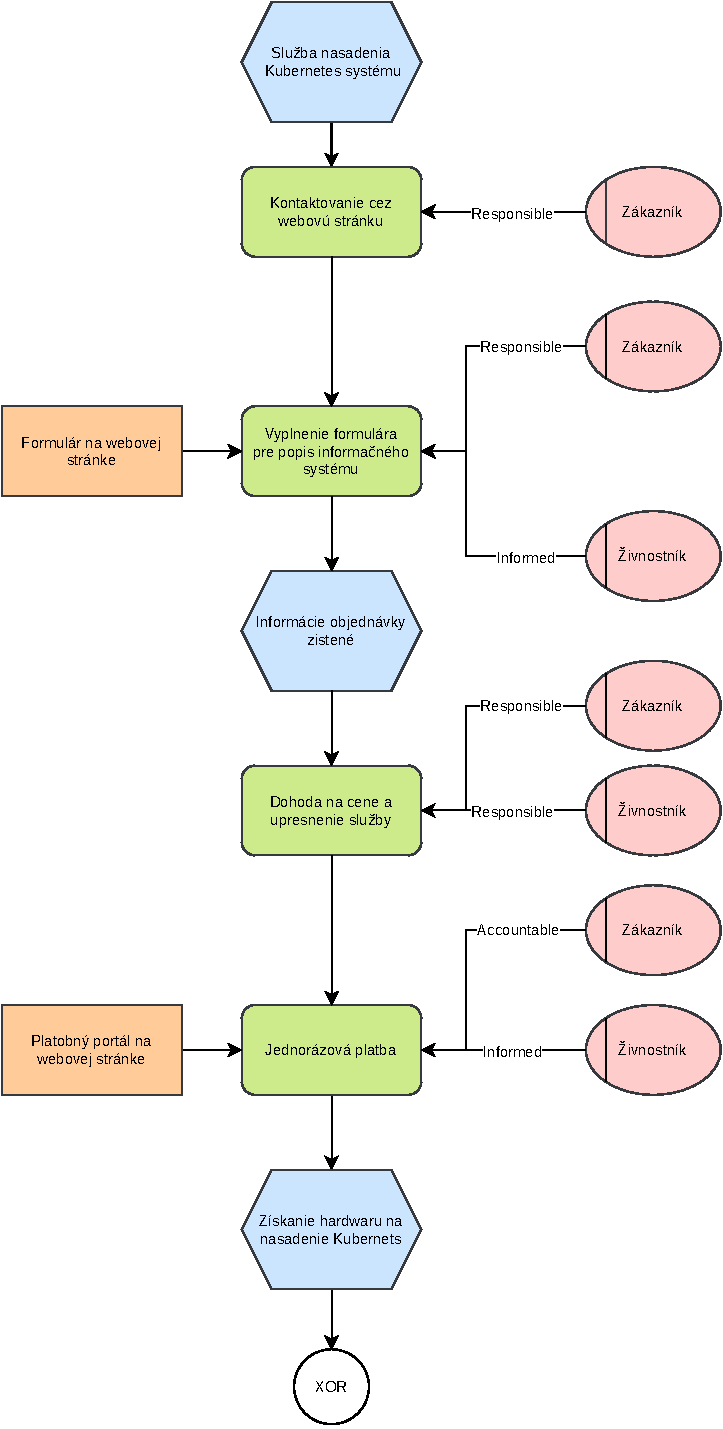
\includegraphics[width=0.5\textwidth]{images/EPC_1.pdf}
  \caption{EPC Prvá časť}
  \label{ecc:1}
\end{figure}

\begin{figure}[htbp]
  \centering
  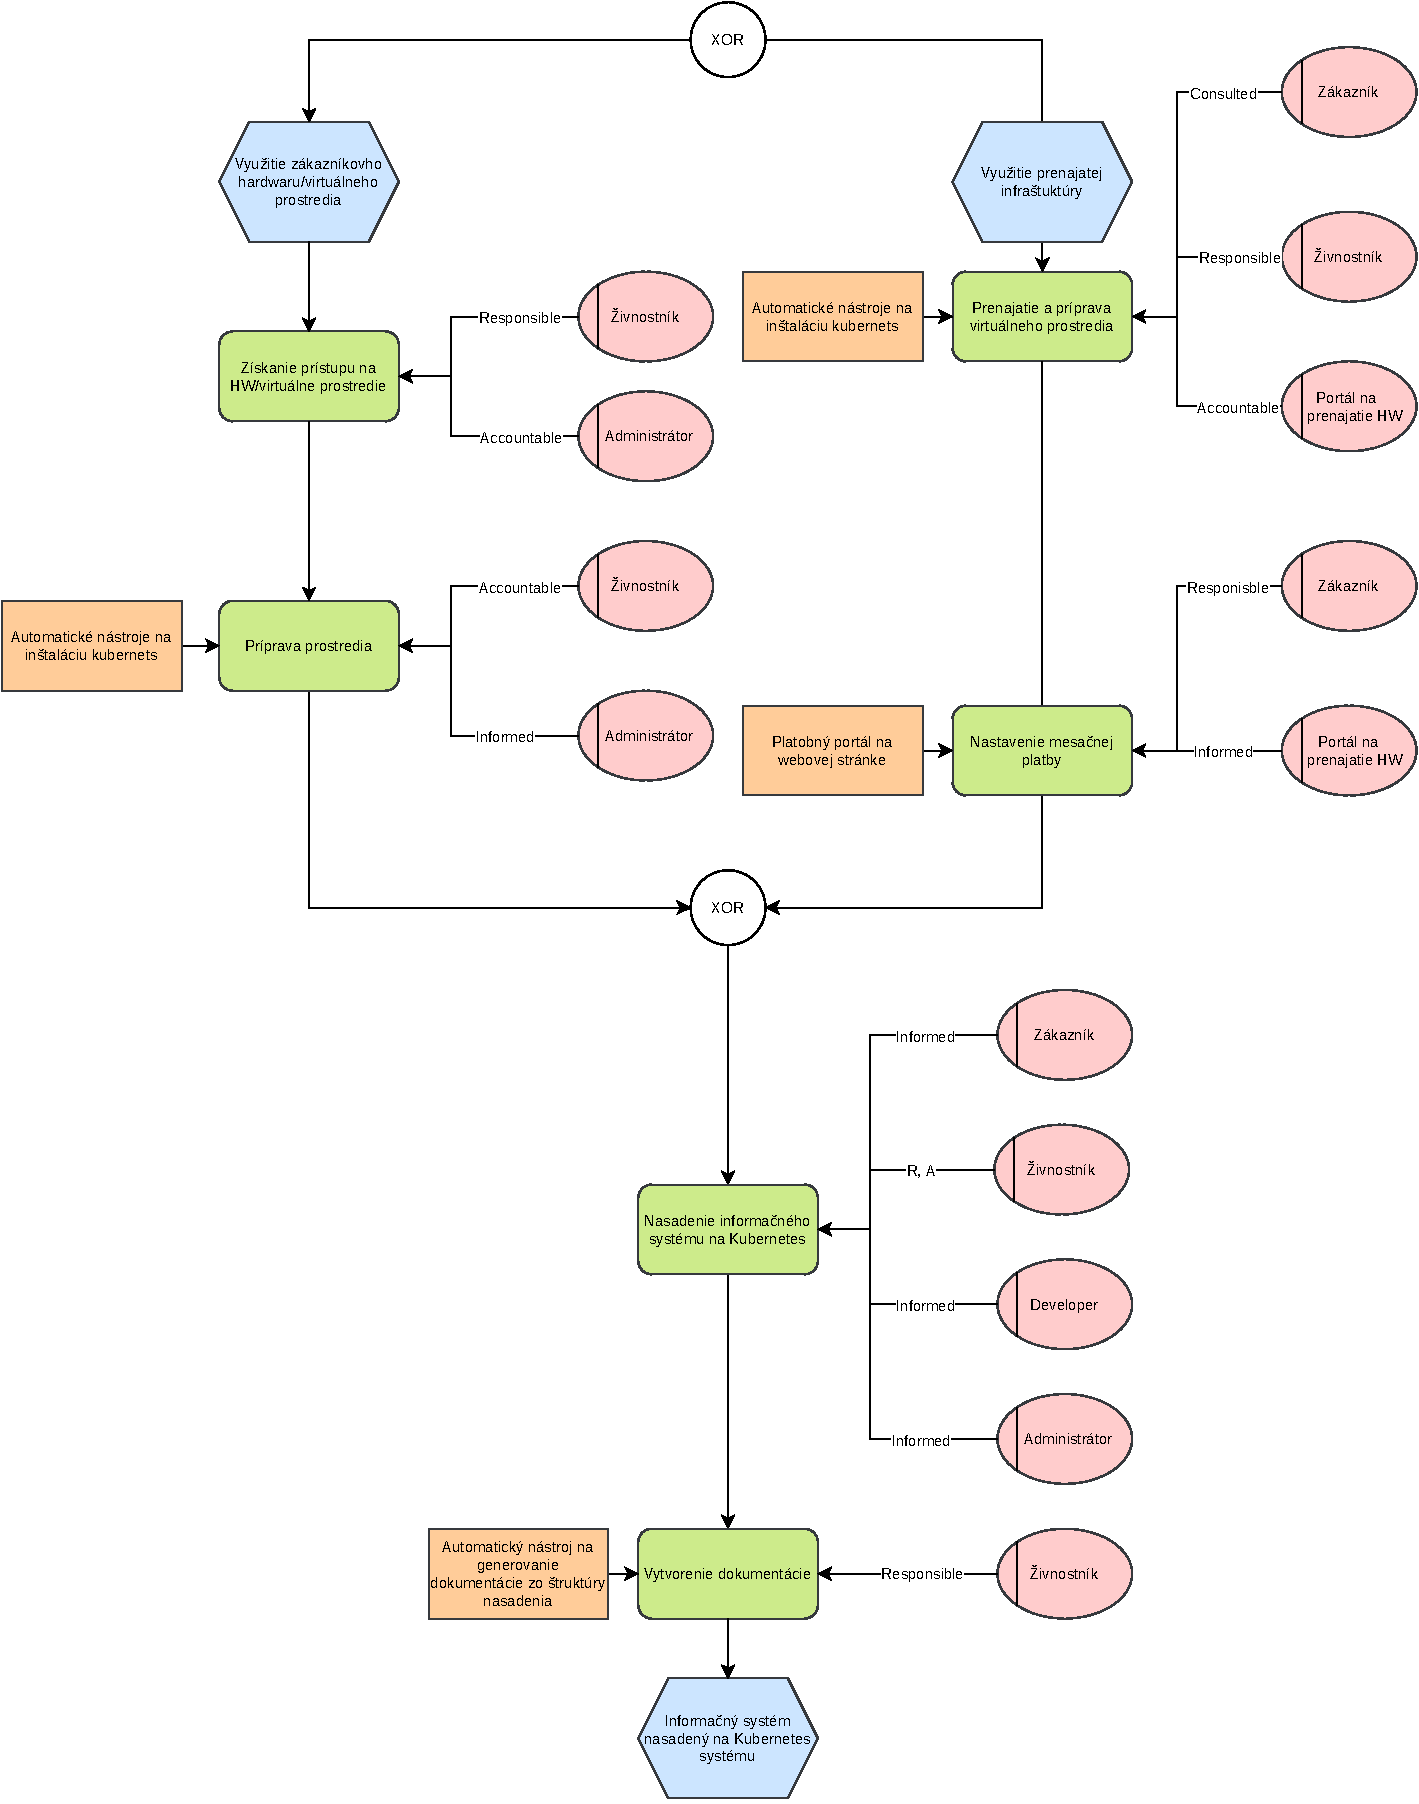
\includegraphics[width=\textwidth]{images/EPC_2.pdf}
  \caption{EPC Druhá časť}
  \label{ecc:2}
\end{figure}

\begin{figure}[htbp]
  \centering
  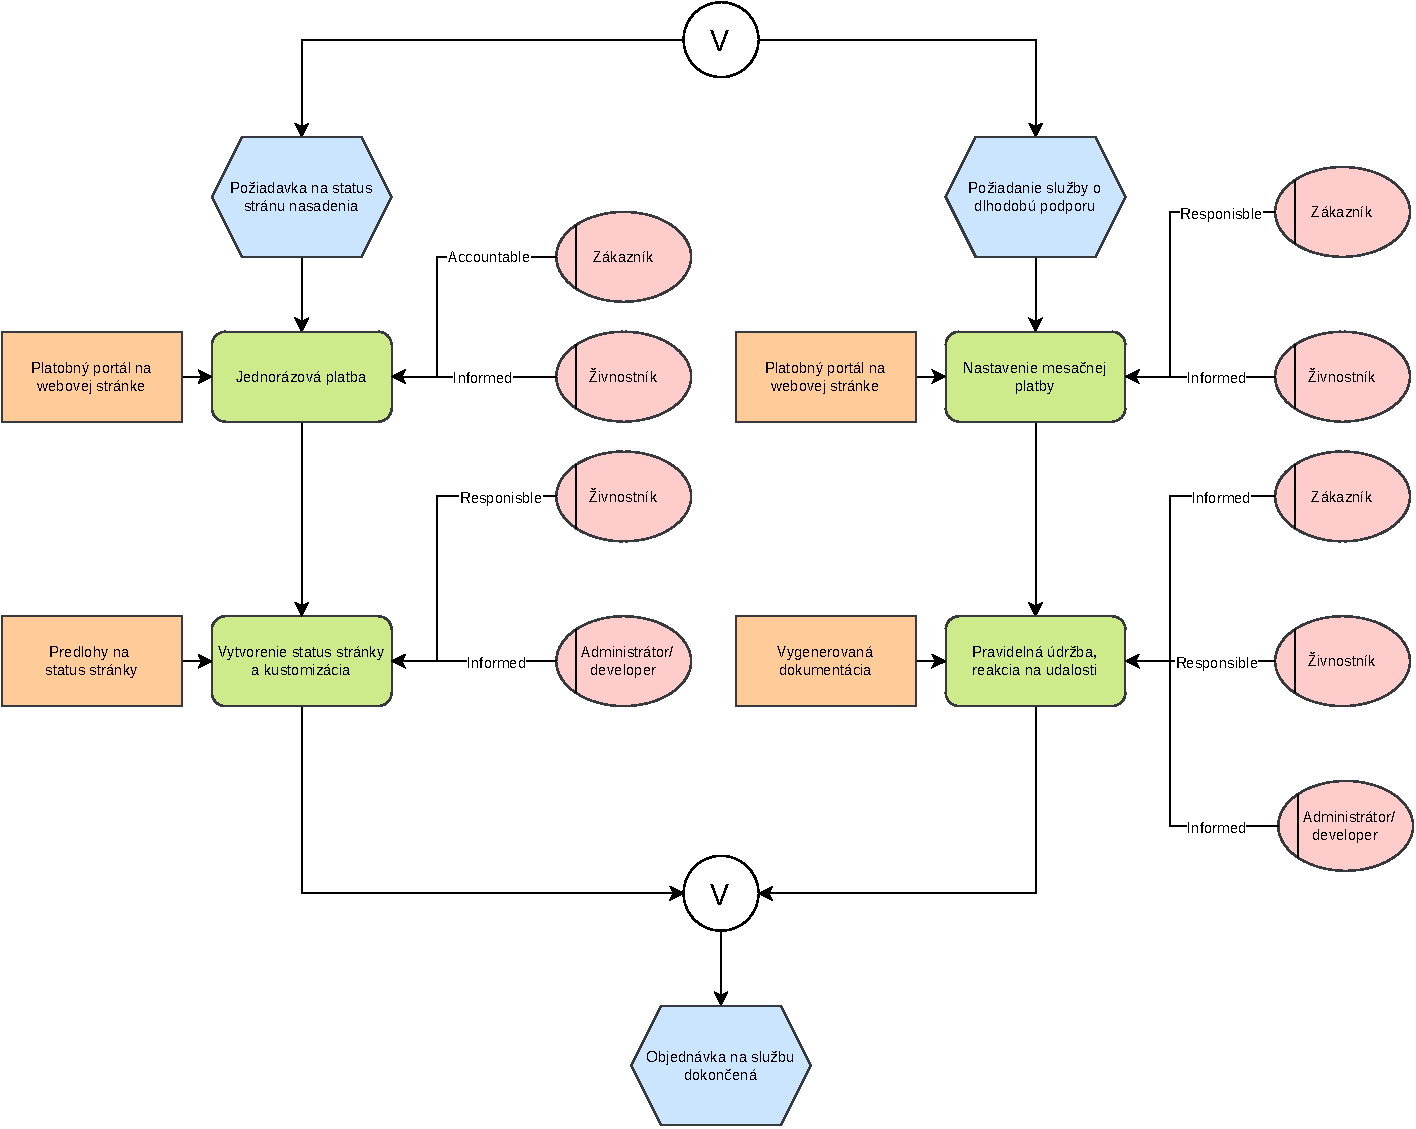
\includegraphics[width=\textwidth]{images/EPC_3.pdf}
  \caption{EPC Tretia časť}
  \label{ecc:3}
\end{figure}

\begin{landscape}
\begin{table}[htbp]
  \centering
  \begin{tabular}{|l|c|c|c|c|c|c|}
      \hline
      & \multirow{2}*{\textbf{Procesné role}} & \multirow{4}*{\textbf{Živnostník}} & \multirow{4}*{\textbf{Zákazník}} & \multirow{4}*{\textbf{Administrátor}} & \multirow{4}*{\textbf{Developer}} & \multirow{4}*{\textbf{HW portál}}\\
       &  &  &  &  &  & \\
       \cline{1-2}\multirow{2}*{\textbf{Popis aktivity}} &  &  &  &  &  & \\
       &  &  &  &  &  & \\
      \hline 
      \multicolumn{2}{|l|}{Kontaktovanie cez webovú stránku} &  & R &  &  & \\
      \hline 
      \multicolumn{2}{|l|}{Vyplnenie formulára pre popis informačného systému} & I & R &  &  & \\
      \hline 
      \multicolumn{2}{|l|}{Dohoda na cene a upresnenie služby} & R & R &  &  & \\
      \hline 
      \multicolumn{2}{|l|}{Jednorázová platba} & I & A &  &  & \\
      \hline 
      \multicolumn{2}{|l|}{Získanie prístupu na HW/virtuálne prostredie} & R &  & A &  & \\
      \hline 
      \multicolumn{2}{|l|}{Príprava prostredia} & A &  & I &  & \\
      \hline 
      \multicolumn{2}{|l|}{Prenajatie a príprava virtuálneho prostredia} & R & C &  &  & A\\
      \hline 
      \multicolumn{2}{|l|}{Nastavenie mesačnej platby} &  & R &  &  & I\\
      \hline 
      \multicolumn{2}{|l|}{Nasadenie informačného systému na Kubernetes} & R, A & I & I & I & \\
      \hline 
      \multicolumn{2}{|l|}{Vytvorenie dokumentácie} & R &  &  &  & \\
      \hline 
      \multicolumn{2}{|l|}{Vytvorenie status stránky a kustomizácia} & R &  & I &  & \\
      \hline 
      \multicolumn{2}{|l|}{Pravidelná údržba, reakcia na udalosti} & R & I & I &  & \\
      \hline 
  \end{tabular}
  \caption{RACI matica}
  \label{raci}
\end{table}
\end{landscape}


\chapter{Výber systému}
\label{ch:vyber}
Systém pomocou ktorého budem ponúkať služby si naprogramujem sám keďže jeho obsah bude relatívne malý. Bude sa skladať z nasledovných častí:

\begin{itemize}
  \item Formulár na vyplnenie objednávky
  \item Platobná brána pre jednorázovú platbu
  \item Platobná brána pre opakovanú platbu
  \item Stránka z popisom mojich služieb
\end{itemize}

Na implementáciu samotnej web aplikácie pre zákazníkov použijem Vue \cite{vue} a Node.js \cite{Node} javascript frameworky. Databáza nebude potrebná keďže stránka nebude použivať žiadne perzistentné dáta.

Namiesto databáze v aplikácií pre zákazníkov implementujem jednoduchý informačný systém pre moje vnútorné použitie ktorý bude naprogramovaný z rovnakými frameworkami. Systém buďe obsahovať databázový systém ktorý bude udržiavať konkrétne objednávky a ich stav. Prvotný stav objednávky bude vytvorený pomocou web aplikácie po vyplnení formulára. Dáta objednávky sa budú posielať pomocou REST API rozhrania do môjho informačného systému kďe sa ďalej spracujú. Ďalšie zmeny objednávky bude možné upraviť pomocou aplikácie pre vnútorné použitie. 

Toto riešenie som si vybral pretože mám skúsenosti z web developmentom a neoplatí sa mi prenajímať celí e-shop keďže ponúkam služby a nie fyzický produkt.

\section{Výber virtuálneho prostredia}
\label{vyber}

Aby bola moja webová aplikácie pre zákazníkov dostupná, budem si musieť prenajať virtuálny server kde nasadím môj systém. Nebudem potrebovať veľký výkon keďže očakávam že na začiatku nebude počet objednávok veľký. Ak sa počet návštev zväčší, použijem lepšie parametre. Tabuľka \ref{serveri} popisuje kritéria výberu jednotlivých systémov. Pre každý systém som si zvolil tieto alebo podobné parametre:

\begin{itemize}
  \item CPU -- 2 jadrá
  \item CPU frekvencia -- 2-2.5\,Ghz
  \item Disk -- 20-50\,GB
\end{itemize}

Každá hodnota je bodovaná stupnicou 0 po 5. V prvom stĺpci je súčet všetkých hodnotení v riadku. Hodnotenie stĺpcov Cena, RAM a prenos dát sú hodnotené podla tabuľky \ref{serveri_2}. Ostatné stĺpce sú hodnotené bez stupnice a hodnoty sú určené podla môjho zváženia. Tieto stĺpce môžu mať aj negatívne hodnoty do -5. Z tabuľky \ref{serveri} je zrejmé že \textbf{Linode} vyhráva a budem ho teda používať ako virtuálny server pre moju stránku.

\begin{landscape}
  \begin{table}[h!]
    \centering
    \begin{tabular}{|c|l|c|c|c|c|c|c|}
      \hline
      Body   & Názov            & Cena za mesiac         & RAM       & Prenos dát  & In/Out rýchlosť  & Poznámka          \\
      \hline
      (23.5) & \textbf{Linode}  & 10.14\,\texteuro\ (15) & 2\,GB (3) & 2 TB (4.5)  & 40/1 Gbps (4)    & Zdielané CPU (-3) \\
      \hline
      (22.5) & Kametra          & 6.08\,\texteuro\ (15)  & 2\,GB (3) & 1 TB (4.5)  & 10/10 Gbps (3)   & Zdielané CPU (-3) \\
      \hline
      (18.5) & Liquidweb        & 25.35\,\texteuro\ (9)  & 2\,GB (3) & 10 TB (7.5) & - (-1)           & - (0)             \\
      \hline
      (21)   & CloudSigma       & 20\,\texteuro\ (12)    & 4\,GB (4) & 5 TB (6)    & - (-1)           & - (0)             \\
      \hline
      (20)   & Amazon Ligthsail & 20.28\,\texteuro\ (9)  & 4\,GB (4) & 3 TB (6)    & 900/900 Mbps (1) & - (0)             \\
      \hline
      (21)   & Vultr            & 20.28\,\texteuro\ (9)  & 4\,GB (4) & 3 TB (6)    & 2/2 Gbps (2)     & - (0)             \\
      \hline
    \end{tabular}
    \caption{Porovnanie ponúk}
    \label{serveri}
  \end{table}
\end{landscape}


\begin{table}[h!]
  \centering
  \begin{tabular}{|c|c|c|c|c|c|c|}
    \hline
    Názov      & Váha & 1                    & 2                   & 3                   & 4                   & 5                  \\
    \hline
    Cena       & 3    & $>=$75.01\,\texteuro & 75-40.01\,\texteuro & 40-20.01\,\texteuro & 20-15.01\,\texteuro & 15-0.01\,\texteuro \\
    RAM        & 1    & 0.5\,GB              & 1\,GB               & 2\,GB               & 4\,GB               & 8\,GB              \\
    Prenos dát & 1.5  & $<=$500\,GB          & 501-1000\,GB        & 1-2\,TB             & 2-5\,TB             & $>$5\,TB           \\
    \hline
  \end{tabular}
  \caption{Stupnice pre vybrané stĺpce}
  \label{serveri_2}
\end{table}



\chapter{Implementácia systému}


\chapter{Prevádzka systému}

V nasledujúcich sekciách je popísaná prevádzka systému. Konkrétnejšie zálohovanie a obnovy pri havárií, dostupnosť a administratíva webových aplikácií.

\section{Bezpečnosť dát}
\label{sec}
Ako som spomínal v kapitole \ref{ch:vyber} informačný systém bude tvorený dvoma aplikáciami a informácie si budú vymieňať pomocou REST API. Zabezpečenie pre toto API bude tvorené pomocou API kľúča ktorý bude dostupný iba mne aby náhodný ľudia na internete nemohli meniť alebo čítať moje objednávky.

Zálohovanie databázového systému prístupného len mňe budem riešiť pravidlom 3 2 1. Budú existovať 3 zálohy:
\begin{itemize}
  \item Záloha na systéme na ktorom beží aj systém
  \item Záloha na externom úložisku u mňa doma (NAS)
  \item Záloha na cloude MEGA
\end{itemize}
Zálohy sa budú vytvárať každý ďen automaticky a budú sa ukladať na všetky 3 spôsoby záloh. Úložiská budú udržiavať zálohy po dobu jedného mesiaca. V prípade havárie budú použité najaktuálnejšie dáta na obnovu obidvoch webových aplikácií.


\section{Dostupnosť}

Zákaznícka podpora bude dostupná pomocou emailového kontaktu alebo v súrnych prípadoch telefonického/video-hovorového kontaktu. Podpora bude dostupná zo začiatku môjho živnostníctva v prevádzkovej dobe, čo sú všetky pracovné dni od 8:00 do 16:00. Neskoršie by som nabral ďalších zamestnancov ktorý budú poskytovať 24/7/365 podporu a budú ma kontaktovať len pri vážnych problémoch.

Samotný systém bude dostupný stále a lehota odpovedania na objednávku bude jeden týždeň.

\section{Administratíva systému a objednávok}

Samotný kód pre webové aplikácie bude spravovaný verzovacím systémom git. Kód bude ukladaný na službe GitHub kde repozitár bude nastavený ako privátny. Ako administrátor a developer systému sa budem starať o bezpečnosť systému popísanú v sekcii \ref{sec}. Periodicky budem taktiež sledovať stav systémov, či všetko funguje ako má.


\begin{thebibliography}{99}

  \bibitem{vue}
  \textit{Vue} [online]. [cit. 2022-10-23]. Dostupné z: \url{https://vuejs.org/}
  \bibitem{Node}
  \textit{NodeJS} [online]. [cit. 2022-10-23]. Dostupné z: \url{https://nodejs.org/en/}

\end{thebibliography}


%% Konec dokumentu
\end{document}
